% Options for packages loaded elsewhere
% Options for packages loaded elsewhere
\PassOptionsToPackage{unicode}{hyperref}
\PassOptionsToPackage{hyphens}{url}
\PassOptionsToPackage{dvipsnames,svgnames,x11names}{xcolor}
%
\documentclass[
  conference]{IEEEtran}
\usepackage{xcolor}
\usepackage{amsmath,amssymb}
\setcounter{secnumdepth}{5}
\usepackage{iftex}
\ifPDFTeX
  \usepackage[T1]{fontenc}
  \usepackage[utf8]{inputenc}
  \usepackage{textcomp} % provide euro and other symbols
\else % if luatex or xetex
  \usepackage{unicode-math} % this also loads fontspec
  \defaultfontfeatures{Scale=MatchLowercase}
  \defaultfontfeatures[\rmfamily]{Ligatures=TeX,Scale=1}
\fi
\usepackage{lmodern}
\ifPDFTeX\else
  % xetex/luatex font selection
\fi
% Use upquote if available, for straight quotes in verbatim environments
\IfFileExists{upquote.sty}{\usepackage{upquote}}{}
\IfFileExists{microtype.sty}{% use microtype if available
  \usepackage[]{microtype}
  \UseMicrotypeSet[protrusion]{basicmath} % disable protrusion for tt fonts
}{}
\makeatletter
\@ifundefined{KOMAClassName}{% if non-KOMA class
  \IfFileExists{parskip.sty}{%
    \usepackage{parskip}
  }{% else
    \setlength{\parindent}{0pt}
    \setlength{\parskip}{6pt plus 2pt minus 1pt}}
}{% if KOMA class
  \KOMAoptions{parskip=half}}
\makeatother
% Make \paragraph and \subparagraph free-standing
\makeatletter
\ifx\paragraph\undefined\else
  \let\oldparagraph\paragraph
  \renewcommand{\paragraph}{
    \@ifstar
      \xxxParagraphStar
      \xxxParagraphNoStar
  }
  \newcommand{\xxxParagraphStar}[1]{\oldparagraph*{#1}\mbox{}}
  \newcommand{\xxxParagraphNoStar}[1]{\oldparagraph{#1}\mbox{}}
\fi
\ifx\subparagraph\undefined\else
  \let\oldsubparagraph\subparagraph
  \renewcommand{\subparagraph}{
    \@ifstar
      \xxxSubParagraphStar
      \xxxSubParagraphNoStar
  }
  \newcommand{\xxxSubParagraphStar}[1]{\oldsubparagraph*{#1}\mbox{}}
  \newcommand{\xxxSubParagraphNoStar}[1]{\oldsubparagraph{#1}\mbox{}}
\fi
\makeatother


\usepackage{longtable,booktabs,array}
\newcounter{none} % for unnumbered tables
\usepackage{calc} % for calculating minipage widths
% Correct order of tables after \paragraph or \subparagraph
\usepackage{etoolbox}
\makeatletter
\patchcmd\longtable{\par}{\if@noskipsec\mbox{}\fi\par}{}{}
\makeatother
% Allow footnotes in longtable head/foot
\IfFileExists{footnotehyper.sty}{\usepackage{footnotehyper}}{\usepackage{footnote}}
\makesavenoteenv{longtable}
\usepackage{graphicx}
\makeatletter
\newsavebox\pandoc@box
\newcommand*\pandocbounded[1]{% scales image to fit in text height/width
  \sbox\pandoc@box{#1}%
  \Gscale@div\@tempa{\textheight}{\dimexpr\ht\pandoc@box+\dp\pandoc@box\relax}%
  \Gscale@div\@tempb{\linewidth}{\wd\pandoc@box}%
  \ifdim\@tempb\p@<\@tempa\p@\let\@tempa\@tempb\fi% select the smaller of both
  \ifdim\@tempa\p@<\p@\scalebox{\@tempa}{\usebox\pandoc@box}%
  \else\usebox{\pandoc@box}%
  \fi%
}
% Set default figure placement to htbp
\def\fps@figure{htbp}
\makeatother





\setlength{\emergencystretch}{3em} % prevent overfull lines

\providecommand{\tightlist}{%
  \setlength{\itemsep}{0pt}\setlength{\parskip}{0pt}}



 
\usepackage[numbers]{natbib}
\bibliographystyle{IEEEtran}


% IEEE author blocks: pandoc's default template emits a plain \author{}, which
% drops affiliation and email, so the block is defined here instead and the
% `author` key is left out of the notebook front matter. The definition is
% deferred to \AtBeginDocument because the template's own \author{} is written
% after this file is included and would otherwise win.
\AtBeginDocument{%
% conference mode locks out \thanks, silently dropping the footnote, so the
% lockout is overridden before \author is defined
\IEEEoverridecommandlockouts
% two parallel blocks rather than one inline pair, so each email sits under its
% own author's name instead of relying on the two columns happening to align
\author{%
\IEEEauthorblockN{Kiarash Ara}
\IEEEauthorblockA{arak@mcmaster.ca}
\and
\IEEEauthorblockN{Yiheng Wu}
\IEEEauthorblockA{wu1261@mcmaster.ca}%
\thanks{Both authors are with the School of Computational Science and
Engineering, McMaster University. Course project for CSE 705 Deep Learning,
Summer 2026; instructor Dr.~Anwar Mirza.}%
}%
}

% IEEE body text runs with indented paragraphs and no inter-paragraph skip;
% pandoc's default leaves a visible gap that costs vertical space in a
% page-limited format
\setlength{\parskip}{0pt}
\setlength{\parindent}{1em}
\makeatletter
\@ifpackageloaded{caption}{}{\usepackage{caption}}
\AtBeginDocument{%
\ifdefined\contentsname
  \renewcommand*\contentsname{Table of contents}
\else
  \newcommand\contentsname{Table of contents}
\fi
\ifdefined\listfigurename
  \renewcommand*\listfigurename{List of Figures}
\else
  \newcommand\listfigurename{List of Figures}
\fi
\ifdefined\listtablename
  \renewcommand*\listtablename{List of Tables}
\else
  \newcommand\listtablename{List of Tables}
\fi
\ifdefined\figurename
  \renewcommand*\figurename{Fig.}
\else
  \newcommand\figurename{Fig.}
\fi
\ifdefined\tablename
  \renewcommand*\tablename{TABLE}
\else
  \newcommand\tablename{TABLE}
\fi
}
\@ifpackageloaded{float}{}{\usepackage{float}}
\floatstyle{ruled}
\@ifundefined{c@chapter}{\newfloat{codelisting}{h}{lop}}{\newfloat{codelisting}{h}{lop}[chapter]}
\floatname{codelisting}{Listing}
\newcommand*\listoflistings{\listof{codelisting}{List of Listings}}
\makeatother
\makeatletter
\makeatother
\makeatletter
\@ifpackageloaded{caption}{}{\usepackage{caption}}
\@ifpackageloaded{subcaption}{}{\usepackage{subcaption}}
\makeatother
\usepackage{bookmark}
\IfFileExists{xurl.sty}{\usepackage{xurl}}{} % add URL line breaks if available
\urlstyle{same}
\hypersetup{
  pdftitle={Architecture-Dependent Failure Modes in Deep Graph Neural Networks: Separating Oversmoothing from Optimization Failure},
  colorlinks=true,
  linkcolor={blue},
  filecolor={Maroon},
  citecolor={Blue},
  urlcolor={Blue},
  pdfcreator={LaTeX via pandoc}}


\title{Architecture-Dependent Failure Modes in Deep Graph Neural
Networks: Separating Oversmoothing from Optimization Failure}
\author{}
\date{}
\begin{document}
\maketitle
\begin{abstract}
Graph neural networks lose the ability to discriminate between nodes as
depth increases, a phenomenon usually attributed to oversmoothing.
Accuracy alone cannot establish that attribution: a deep model may
instead fail because optimization never moves its weights. We compare
GCN, GraphSAGE, GAT, and GCNII on the Cora citation network at depths 2,
4, 8, 16, and 32, recording Dirichlet energy and mean average distance
(MAD) at three capture points per run, initialization, the selected
checkpoint, and the final epoch, over 534 runs at ten seeds. Depth-32
failure is architecture-dependent rather than one shared mechanism.
GraphSAGE and GAT do not train at depth 32: their training loss stays
within 0.02 nats of the uninformed floor \(\ln 7 = 1.9459\) and their
checkpoint state stays near initialization. GCN partially trains,
reaching 24.07\% accuracy, below the 31.9\% majority-class floor, and
develops early-layer energy collapse with late-layer growth spanning 26
orders of magnitude across seeds. GraphSAGE's metrics dissociate: MAD
falls to near zero by depth 4 while energy plateaus near 19, because it
collapses onto the constant direction, outside the augmented Laplacian's
degree-weighted null space. Jumping Knowledge restores GCN to 73.13\%
and GAT to 72.09\% but GraphSAGE to only 40.47\%; GCNII alone improves
with depth, reaching 83.26\%.
\end{abstract}


\begin{IEEEkeywords}
graph neural networks, oversmoothing, network depth, Dirichlet energy,
node classification, trainability
\end{IEEEkeywords}

\section{Introduction}\label{introduction}

Many systems of practical interest are described more faithfully as
graphs than as collections of independent observations: citation
networks connect papers through references, recommendation systems
connect users to items, and molecular graphs connect atoms through
bonds. Graph neural networks (GNNs) exploit this structure through
message passing, in which each node updates its representation by
combining its own features with information aggregated from its
neighbors \citep{gilmer2017neural}.

Depth is the mechanism by which a GNN widens its receptive field. One
message-passing layer reaches direct neighbors, two reach
neighbors-of-neighbors, and an \(L\)-layer model can draw on information
from roughly \(L\) hops away. In practice, adding layers tends to make
GNNs harder to train and reduces their ability to separate classes:
repeated aggregation drives node representations toward one another
until they become indistinguishable, a behavior commonly called
oversmoothing \citep{li2018deeper, oono2020graph}. Depth is not a
tunable convenience in every domain. In physics-informed graph learning,
where a discretized mesh is treated as a graph, a useful prediction
requires information to cross enough of the domain, so the depth at
which representations degrade constrains whether the model is applicable
at all.

\subsection{The Attribution Problem}\label{the-attribution-problem}

Oversmoothing is frequently invoked as though it were the only reason a
deep GNN fails, but a decrease in accuracy does not establish that
representations have collapsed. A deep model can also fail because
optimization becomes ineffective, because gradients vanish, or because
neighborhood information is compressed past usefulness. These mechanisms
can produce nearly identical accuracy curves while leaving very
different signatures in the hidden representations. A model that trained
and then collapsed and a model whose weights never moved are separated
by their internal state, not by their test accuracy.

We therefore separate two terms and use them consistently.
\emph{Oversmoothing} names a mechanism, the contraction of
representations toward one another under repeated propagation.
\emph{Collapse} names what the metrics register when it happens.
Oversmoothing is a claim about cause; collapse is a claim about what was
measured, and establishing the first from the second requires ruling out
the alternative that nothing was learned at all.

\subsection{Approach}\label{approach}

We study semi-supervised node classification on Cora
\citep{sen2008collective, yang2016revisiting}, holding dataset, split,
and training protocol fixed so that depth is the only variable that
moves. Four architectures with materially different aggregation rules
are compared: GCN \citep{kipf2017semi}, GraphSAGE
\citep{hamilton2017inductive}, GAT \citep{velickovic2018graph}, and
GCNII \citep{chen2020simple}, each at depths 2, 4, 8, 16, and 32 over
ten seeds.

Each run is additionally instrumented at the representation level with
Dirichlet energy and mean average distance (MAD)
\citep{chen2020measuring}, reported as a pair because they are invariant
to different things. Both are captured at three points in every run: at
initialization before any gradient step, at the checkpoint selected by
lowest validation loss, and at the final epoch. The epoch-0 capture
isolates the architecture from the optimizer, and the
epoch-0-to-checkpoint comparison is what separates a trained state from
an untrained one.

\subsection{Contributions}\label{contributions}

\begin{itemize}
\tightlist
\item
  \textbf{An architecture-resolved account of depth-32 failure}, showing
  that GCN, GraphSAGE, and GAT fail through distinct mechanisms rather
  than one shared collapse, separated by measurements that do not depend
  on accuracy.
\item
  \textbf{A three-capture diagnostic protocol} distinguishing collapse
  present at initialization from collapse that develops during training,
  applied uniformly across 534 runs.
\item
  \textbf{A measured explanation of metric dissociation}: GraphSAGE
  collapses onto the constant direction, which lies outside the
  augmented Laplacian's degree-weighted null space, so its energy cannot
  vanish however completely its directions align.
\item
  \textbf{An ablation of three mitigations and their combination} at
  depth 32, showing that the most effective one is
  architecture-dependent rather than universal.
\end{itemize}

The study is confined to Cora and its standard public split, so the
depth at which performance declines and the ranking of mitigations
should not be assumed to transfer. Per-layer gradient norms are not
recorded, so explanations appealing to gradient behavior are stated as
consistent with the measurements rather than established by them.

\section{Related Work}\label{related-work}

\subsection{Message Passing and Depth}\label{message-passing-and-depth}

Most modern GNNs are instances of the message-passing framework
\citep{gilmer2017neural}, differing in the aggregation rule. GCN applies
a symmetrically normalized adjacency operator \citep{kipf2017semi};
GraphSAGE transforms the node and the neighborhood mean through separate
weight matrices and was introduced for inductive settings
\citep{hamilton2017inductive}; GAT replaces fixed degree weights with
learned attention \citep{velickovic2018graph}. Because depth determines
how far information travels, these differing rules are also differing
answers to what repeated application does to a representation.

\subsection{Oversmoothing and Its
Measurement}\label{oversmoothing-and-its-measurement}

Li, Han, and Wu identified graph convolution as a form of Laplacian
smoothing and showed that the operation letting neighbors share
information eventually makes them indistinguishable
\citep{li2018deeper}. Oono and Suzuki strengthened this into an
asymptotic statement: under conditions on the weight spectra, deep GNN
representations approach a low-dimensional invariant subspace
exponentially in depth \citep{oono2020graph}. Cai and Wang recast the
phenomenon in terms of Dirichlet energy, which contracts
multiplicatively at a rate governed by the weight norms and the graph
spectral gap \citep{cai2020note}. These results establish that
contraction happens; they do not establish that a given model's poor
accuracy was caused by it.

Chen et al.~propose MAD, the mean pairwise cosine distance among node
representations, together with MADGap, which correlates with test
accuracy closely enough to serve as a training-free quality predictor
\citep{chen2020measuring}. That correlation is precisely why this study
reports MAD but not MADGap: a metric validated as an accuracy predictor
cannot then be used to ask whether collapse and poor accuracy are
separable.

\subsection{Trainability}\label{trainability}

Depth degrades GNNs through routes other than smoothing. Kipf and
Welling report a depth study in an appendix rather than in their main
results, finding best performance at two to three layers and training
becoming difficult beyond roughly seven layers without residual
connections \citep{kipf2017semi}. That is a statement about
optimization, not about representation collapse, and it is the prior
finding this work extends.

\subsection{Mitigations}\label{mitigations}

Residual connections add an identity path that preserves an earlier
representation and shortens the gradient route. PairNorm instead acts on
the geometry directly, centering and rescaling rows so their dispersion
does not shrink with depth \citep{zhao2020pairnorm}. Jumping Knowledge
changes the readout rather than the propagation, combining
representations from several depths \citep{xu2018representation}. GCNII
modifies the layer itself, adding an initial-residual term and an
identity mapping \citep{chen2020simple}.

\subsection{The Gap}\label{the-gap}

Prior work establishes that accuracy declines with depth and,
separately, that representations contract with depth. What is rarely
established is that the first was caused by the second in a particular
model. Evaluations typically report a single collapse metric at a single
point in training, usually the trained model, which cannot separate a
network that trained and then collapsed from one whose weights never
left initialization. This study addresses that gap by holding dataset,
split, and protocol fixed across four architectures, reporting two
metrics with different invariances as a pair, and capturing both at
three points so the untrained state is an explicit reference.

\section{Methodology}\label{methodology}

\subsection{Data and Task}\label{data-and-task}

All experiments use the Cora citation network through PyTorch
Geometric's \texttt{Planetoid} loader
\citep{sen2008collective, yang2016revisiting}: 2,708 papers,
1,433-dimensional binary bag-of-words features, seven classes, and the
standard public split of 140 training, 500 validation, and 1,000 test
nodes. The training set holds 20 labeled papers per class. Features are
row-normalized, matching the published GCN setup \citep{kipf2017semi}.
Every node participates in message passing regardless of split; only
training-node labels enter the loss.

Let \(G=(V,E)\) with \(|V|=N\), feature matrix
\(X\in\mathbb{R}^{N\times F}\), and adjacency \(A\). Self-loops are
added, \(\widetilde{A}=A+I\), with augmented degrees
\(\widetilde{d}_i=\sum_j \widetilde{A}_{ij}\) and
\(\widetilde{D}=\operatorname{diag}(\widetilde{d}_1,\ldots,\widetilde{d}_N)\).
The normalized propagation operator and Laplacian are

\[
\widehat{A}=\widetilde{D}^{-1/2}\widetilde{A}\widetilde{D}^{-1/2},
\qquad
\mathcal{L}=I-\widehat{A}.
\]

\subsection{Architectures}\label{architectures}

Four update rules are compared. GCN \citep{kipf2017semi} applies

\[
H^{(\ell+1)}=\sigma\!\left(\widehat{A}H^{(\ell)}W^{(\ell)}\right),
\qquad H^{(0)}=X .
\]

GraphSAGE with mean aggregation \citep{hamilton2017inductive} transforms
the node and its neighborhood mean
\(m_i^{(\ell)}=|\mathcal{N}(i)|^{-1}\sum_{j\in\mathcal{N}(i)}h_j^{(\ell)}\)
separately,

\[
h_i^{(\ell+1)}=\sigma\!\left(W_{\mathrm{self}}^{(\ell)}h_i^{(\ell)}+W_{\mathrm{neigh}}^{(\ell)}m_i^{(\ell)}+b^{(\ell)}\right).
\]

GAT \citep{velickovic2018graph} replaces fixed weights with attention.
With \(q_i^{(\ell)}=W^{(\ell)}h_i^{(\ell)}\) and
\(e_{ij}^{(\ell)}=\operatorname{LeakyReLU}\!\left((a^{(\ell)})^{T}[q_i^{(\ell)}\Vert q_j^{(\ell)}]\right)\),

\[
\alpha_{ij}^{(\ell)}=\frac{\exp\!\left(e_{ij}^{(\ell)}\right)}{\sum_{k\in\mathcal{N}(i)\cup\{i\}}\exp\!\left(e_{ik}^{(\ell)}\right)} .
\]

GCNII \citep{chen2020simple} adds an initial residual and an identity
mapping,

\[
H^{(\ell+1)}=\sigma\!\left(\Big[(1-\alpha_\ell)\widehat{A}H^{(\ell)}+\alpha_\ell H^{(0)}\Big]\Big[(1-\beta_\ell)I+\beta_\ell W^{(\ell)}\Big]\right),
\]

with \(\alpha=0.1\) and \(\theta=0.5\) from the original paper. Its two
required linear projections are placed outside the counted depth \(L\),
so that \(L\) denotes the same number of message-passing hops for all
four architectures. The known cost is two extra parameterized layers,
bounded in size and independent of depth, which can only overstate
GCNII's capacity relative to its peers.

All four are realized as one parameterized model in which
\texttt{convType} selects the convolution and depth, width, mitigation
hooks, and the recording position are otherwise identical, so a measured
difference is attributable to the convolution. Hidden width is 64
throughout rather than each architecture's published width, because
capacity parity is a precondition for comparing at matched depth: at
width 16, GAT's eight heads would attend over two-dimensional keys.

\subsection{Mitigations}\label{mitigations-1}

Three mitigations attach to the shared layer loop by composition. A
residual connection adds an identity path,
\(H^{(\ell+1)}=F^{(\ell)}(H^{(\ell)})+H^{(\ell)}\), applicable only
where widths match. PairNorm \citep{zhao2020pairnorm} centers and
rescales rows,

\[
\widetilde{H}=H-\tfrac{1}{N}\mathbf{1}\mathbf{1}^{T}H,
\qquad
h_i^{\mathrm{PN}}=s\,\frac{\widetilde{h}_i}{\lVert\widetilde{h}_i\rVert_2+\varepsilon},
\]

the scale-individual variant (PN-SI). Jumping Knowledge (JK)
\citep{xu2018representation} changes the readout, pooling across depths
elementwise,

\[
H_{\mathrm{JK}}=\max\!\left(H^{(1)},H^{(2)},\ldots,H^{(L)}\right),
\]

followed by a linear classifier.

\subsection{Representation
Diagnostics}\label{representation-diagnostics}

For an embedding matrix \(H\) with rows \(h_i\), the
normalized-Laplacian Dirichlet energy is

\[
E(H)=\frac{1}{2}\sum_{i=1}^{N}\sum_{j=1}^{N}\widetilde{A}_{ij}
\left\lVert \frac{h_i}{\sqrt{\widetilde{d}_i}}-\frac{h_j}{\sqrt{\widetilde{d}_j}} \right\rVert_2^2
=\operatorname{Tr}\!\left(H^{T}\mathcal{L}H\right),
\]

reported per dimension as
\(E_{\mathrm{dim}}(H)=E(H)/\operatorname{dim}(H)\) so that layers of
differing width remain comparable. MAD is the mean cosine distance over
node pairs with nonzero distance \citep{chen2020measuring}.

The two are reported together because they are invariant to different
things. Cosine distance is invariant to positive per-node rescaling: for
\(S=\operatorname{diag}(s_1,\ldots,s_N)\) with \(s_i>0\),
\(\operatorname{MAD}(SH)=\operatorname{MAD}(H)\), so MAD captures
directional alignment and discards magnitude. Dirichlet energy is
quadratic, \(E_{\mathrm{dim}}(cH)=c^2E_{\mathrm{dim}}(H)\), and retains
both. Their disagreement is therefore informative: representations can
align almost completely, driving MAD toward zero, while energy stays
high because the direction they align on is not the Laplacian's
degree-weighted null direction.

Not every stored layer is comparable. \(H^{(0)}\) is excluded as sparse
1,433-dimensional input, and under a last-layer readout \(H^{(L)}\) is
excluded as seven-dimensional logits that cross-entropy shapes directly.
The comparable band is therefore \(\mathcal{B}=\{1,\ldots,L-1\}\), or
\(\{1,\ldots,L\}\) under Jumping Knowledge. Energy is reported relative
to the band's first layer,
\(R_\ell=E_{\mathrm{dim}}(H^{(\ell)})/E_{\mathrm{dim}}(H^{(\ell_0)})\)
with \(\ell_0=\min(\mathcal{B})\), and summarized by a contraction slope
\(b\) fitted as

\[
\log\max\!\left\{E_{\mathrm{dim}}\!\left(H^{(\ell)}\right),\varepsilon_E\right\}\approx a+b\ell,
\qquad \varepsilon_E=10^{-12},
\]

the floor guarding against \(\log 0\). The floor can pull a slope toward
zero but cannot create a trend that is not present.

\subsection{Three Capture Points}\label{three-capture-points}

Every run is measured three times, each an eval-mode forward pass under
\texttt{torch.no\_grad()}: at epoch 0 before any gradient step, at the
final epoch on the weights the loop ended with, and at the selected
checkpoint after the best validation-loss state is restored. The
final-epoch capture is taken \emph{before} the restore; taken afterward
it would duplicate the checkpoint capture on every run. The epoch-0
capture isolates the architecture from the optimizer, and the
epoch-0-to-checkpoint comparison is what distinguishes a model that
trained and collapsed from one that never trained.

\subsection{Training Protocol and Experiment
Grid}\label{training-protocol-and-experiment-grid}

All runs use Adam \citep{kingma2015adam} with learning rate \(0.01\),
dropout \(0.5\), and weight decay \(5\times10^{-4}\), the configuration
selected once by a depth-2 GCN search and then frozen across every
architecture and depth, so that the depth effect is not confounded with
a hyperparameter effect. Weight decay is applied uniformly across layers
rather than to the first layer only, so regularization strength does not
become an implicit function of depth. Early stopping and checkpoint
selection are both driven by validation loss, with patience 100 and a
ceiling of 1,000 epochs. Patience is held constant across depth: at a
short window, a 32-layer run whose loss plateaus early halts near epoch
12, leaving a flat curve that a slow optimization and an untrainable
architecture would share.

The sweep is organized as six arms totaling 534 runs: an unmitigated
sweep over GCN, GraphSAGE, and GAT (150 runs); a mitigation ablation on
GCN over residual, PairNorm, JK, and PairNorm+residual (200); GCNII
(50); the winning mitigation carried to GraphSAGE and GAT (100); a
fidelity arm at the published width 16 (10); and the hyperparameter
search (24). Depths are \(\{2,4,8,16,32\}\), log-spaced because the
contraction bound predicts exponential decay in depth, and every
configuration is repeated over ten seeds controlling both initialization
and training stochasticity. All runs are CPU, Python 3.14.4, PyTorch
2.13.0, PyTorch Geometric 2.8.0.

\section{Experiments and Results}\label{experiments-and-results}

\subsection{Baseline Reproduction}\label{baseline-reproduction}

Every reported number is regenerated from the stored per-run records,
and results are mean and standard deviation over ten seeds. Before depth
is varied, each architecture is checked at depth 2 against the figure
its own paper reports. GCN reaches 81.49\% (± 0.32) against 81.5\%
\citep{kipf2017semi}; GraphSAGE reaches 80.10\% (± 0.42), for which no
published Cora figure exists \citep{hamilton2017inductive}; GAT reaches
78.90\% (± 1.57) against 83.0\% (± 0.7) \citep{velickovic2018graph}, a
shortfall consistent with the shared configuration, from which its own
published setup differs most.

\subsection{Accuracy Across Depth}\label{accuracy-across-depth}

All three conventional architectures degrade sharply with depth
(Fig.~\ref{fig-accuracy-depth}). The drop is not gradual: each loses 4.4
to 8.4 points between depths 2 and 4, falls steeply between 4 and 8, and
stays low. At depth 32, GCN reaches 24.07\%, GraphSAGE 22.65\%, and GAT
19.66\%, all below the 31.9\% majority-class floor computed from the
test-split label counts; GCN's full ten-seed range there, 21.2\% to
26.2\%, lies entirely below it.

\begin{figure}

\centering{

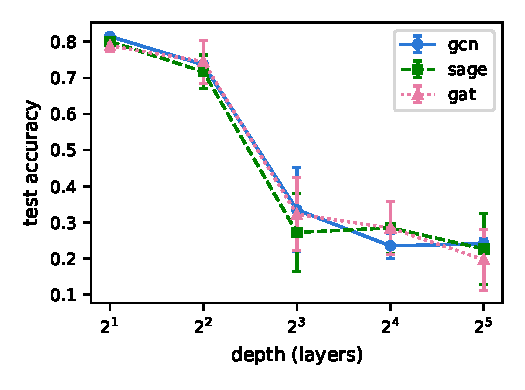
\includegraphics[width=1\linewidth,height=\textheight,keepaspectratio]{../figures/accuracy_vs_depth.pdf}

}

\caption{\label{fig-accuracy-depth}Test accuracy versus depth,
unmitigated GCN, GraphSAGE, and GAT.}

\end{figure}%

Macro-F1 collapses faster still: at depth 32 GAT's is 0.0459 and
GraphSAGE's 0.0514, against GCN's 0.2102, consistent with predictions
concentrating onto a few classes rather than spreading evenly across all
seven.

\subsection{Collapse at
Initialization}\label{collapse-at-initialization}

At epoch 0 the weights are random, so any contraction is attributable to
the architecture rather than to training. GCN and GAT collapse cleanly
in both direction and magnitude, while GraphSAGE collapses in direction
only (Table~\ref{tab:epoch0}). GCN's energy ratio falls about 12 orders
of magnitude by depth 32 and GAT's about 10, consistent with the
multiplicative contraction Cai and Wang describe \citep{cai2020note},
though its numerical tightness is not tested here.

\begin{table*}[t]
\centering
\caption{Epoch-0 MAD and relative energy versus depth, means over ten seeds.
At depth 2 the comparable band holds one layer, so the ratio is not reported.}
\label{tab:epoch0}
\begin{tabular}{llrrrrr}
\hline
Conv & Metric & $d{=}2$ & $d{=}4$ & $d{=}8$ & $d{=}16$ & $d{=}32$\\
\hline
GCN  & MAD                      & 0.600 & 0.240  & 0.085  & 0.023   & 0.0045\\
GCN  & $E_{\text{last}}/E_1$    & ---   & 3.1e-2 & 3.1e-4 & 2.6e-7  & 6.2e-13\\
GAT  & MAD                      & 0.596 & 0.211  & 0.076  & 0.017   & 0.0041\\
GAT  & $E_{\text{last}}/E_1$    & ---   & 7.3e-2 & 2.7e-3 & 1.3e-5  & 1.3e-10\\
SAGE & MAD                      & 0.083 & 1.8e-4 & 9.9e-7 & $\approx$0 & $\approx$0\\
SAGE & $E_{\text{last}}/E_1$    & ---   & 18.3   & 19.8   & 20.3    & 19.3\\
\hline
\end{tabular}
\end{table*}

GraphSAGE's two metrics dissociate at every depth: MAD reaches near zero
by depth 4 while its energy ratio \emph{rises} and then plateaus near
19. A singular-value decomposition at depth 16 over three seeds locates
the cause. GraphSAGE's representation matrix is exactly rank-1
(top-singular-value energy fraction 1.0000), and its top singular vector
matches the constant direction at cosine 1.0000 against 0.9512 to the
\(\sqrt{\text{degree}}\) direction; GCN and GAT are only mostly rank-1
(0.93 to 0.98) and do not separate the two candidates. Because Cora's
degrees run from 2 to 169, the augmented Laplacian's null space is the
\(\sqrt{\text{degree}}\) direction rather than the constant vector, so
GraphSAGE collapses onto a direction outside that null space and its
energy cannot vanish however completely its representations align.

\subsection{Separating Trained from Untrained
Failure}\label{separating-trained-from-untrained-failure}

Training changes the picture, and differently per architecture. At the
selected checkpoint GCN's MAD no longer falls with depth, holding near
0.183 at depth 32, while GraphSAGE's and GAT's remain essentially zero,
close to their own epoch-0 values.

Three independently measured quantities converge for GraphSAGE and GAT.
Their training loss never leaves the uninformed floor
\(\ln 7 = 1.9459\), reaching minima of 1.9343 and 1.9393, a movement of
0.01 to 0.02 nats (Fig.~\ref{fig-loss-curves}); their runs exhaust the
patience of 100 epochs almost immediately, at 102 to 168 and 101 to 121
epochs; and their checkpoint MAD is essentially identical to their
epoch-0 MAD. None is derived from the others, which makes their
agreement convergence rather than circularity: at depth 32 these two
architectures do not train at all.

\begin{figure}

\centering{

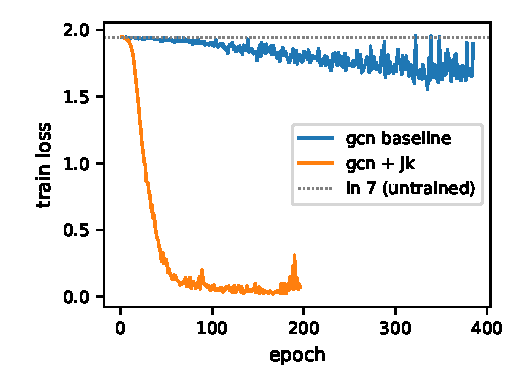
\includegraphics[width=1\linewidth,height=\textheight,keepaspectratio]{../figures/loss_curves_depth32.pdf}

}

\caption{\label{fig-loss-curves}Training loss versus epoch at depth 32,
unmitigated GCN against GCN with Jumping Knowledge; the dotted line
marks \(\ln 7\).}

\end{figure}%

GCN behaves differently. Its loss descends to a mean minimum of 1.57 and
its runs last 315 to 883 epochs. Its checkpoint energy ratio grows
rather than decays, spanning 26 orders of magnitude across seeds at
depth 32, because the \emph{denominator} has collapsed: \(E_1\) falls to
approximately 1.4e-15 and as low as 2.9e-38. For nine of ten seeds the
first 22 to 28 of 31 band layers carry energy below the \(10^{-12}\)
floor while the last few carry very large energy. Depth-32 failure
therefore separates into two training modes, with distinct collapse
signatures inside the non-training pair.

\subsection{Mitigations}\label{mitigations-2}

Jumping Knowledge is the clear winner on GCN, and the ranking does not
carry across architectures (Table~\ref{tab:mitigations}). Residual alone
does not beat the unmitigated baseline at depth 32, and PairNorm
combined with residual is worse than PairNorm alone. Carried to the
other architectures, JK recovers GAT almost to GCN's level including
macro-F1 (0.7252 against 0.7249), but recovers GraphSAGE only to 40.47\%
with macro-F1 0.2611. All ten GraphSAGE+JK seeds sit above the
majority-class floor, so the gain is real, but it is about a third of
what the same mitigation achieves elsewhere and is not spread evenly
across classes. GCNII is the only architecture whose accuracy improves
with depth, and its checkpoint contraction slope stays within roughly
\(\pm 0.4\) at every depth (+0.383, +0.169, −0.037, +0.012) where GCN's
runs from +1.64 to +2.46.

\begin{table}[t]
\centering
\caption{Depth-32 test accuracy for every arm, ten seeds each. GCNII reaches
its best result at the greatest depth tested.}
\label{tab:mitigations}
\begin{tabular}{lrr}
\hline
Configuration & Depth-32 acc. & Macro-F1\\
\hline
GCN, unmitigated            & 24.07\% (\textpm 1.60) & 0.2102\\
GCN + residual              & 19.25\% (\textpm 8.97) & ---\\
GCN + PairNorm              & 58.07\% (\textpm 7.10) & ---\\
GCN + PairNorm + residual   & 24.36\% (\textpm 9.79) & ---\\
GCN + JK                    & \textbf{73.13\%} (\textpm 3.43) & 0.7249\\
GraphSAGE, unmitigated      & 22.65\% (\textpm 9.83) & 0.0514\\
GraphSAGE + JK              & 40.47\% (\textpm 3.76) & 0.2611\\
GAT, unmitigated            & 19.66\% (\textpm 8.46) & 0.0459\\
GAT + JK                    & 72.09\% (\textpm 3.77) & 0.7252\\
GCNII                       & \textbf{83.26\%} (\textpm 0.44) & ---\\
\hline
\end{tabular}
\end{table}

\section{Conclusion and Future Work}\label{conclusion-and-future-work}

Depth-related failure in graph neural networks is
architecture-dependent, and accuracy alone cannot show this. Measuring
Dirichlet energy and MAD at three capture points across 534 runs
separates three behaviors that a single accuracy curve would render
identical. GraphSAGE and GAT do not train at depth 32: their loss never
leaves \(\ln 7\), patience exhausts almost immediately, and their
trained state is close to their untrained one, so attributing their
failure to oversmoothing would be incorrect. GCN partially trains and
develops a distinct signature of early-layer energy collapse paired with
late-layer growth. GCNII alone improves with depth, reaching 83.26\% at
depth 32.

Two results depend on the paired-metric design. GraphSAGE's MAD and
energy disagree at every depth because it collapses onto the constant
direction, which lies outside the degree-weighted null space of Cora's
augmented Laplacian; either metric alone would have misled. And Jumping
Knowledge, the best mitigation on GCN, transfers to GAT but not to
GraphSAGE, so the countermeasure cannot be chosen independently of the
architecture.

The study is limited to one dataset and one split, and per-layer
gradient norms are not recorded, so the mechanism inferred for GCN's
early-layer collapse remains consistent with the measurements rather
than established by them. Adding that instrumentation is the most direct
next step. Two experiments would isolate why GraphSAGE collapses onto
the constant direction at one hop: a degree-normalized-mean variant and
a Glorot-initialized \citep{glorot2010understanding} \texttt{SAGEConv},
run separately. Extending the protocol to graphs with other degree
distributions would show whether the null-space result is Cora-specific.
The protocol, rather than the numbers, is what is expected to transfer.


\bibliography{references.bib}



\end{document}
